\chapter{Script de comparaison de base de donnée}

N'ayant pas de notion de programmation orientée objet\, \footnote{Ce qui sera
enseigné en deuxième année.} je n'ai pas pu rejoindre les développeurs de
l'entreprise dans l'application qu'ils étaient occupés d'effectuer, cela dit on
m'a confié une tâche annexe qui est la comparaison des bases de données.

\begin{figure}
\begin{center}
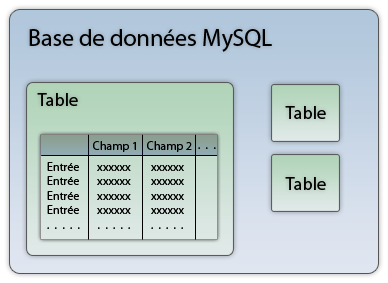
\includegraphics[scale=0.5]{images/bdd.png}
\end{center}
\caption{Un schéma de base de donnée simple.}
\end{figure}

Le besoin premier de ce script est de consulter les différences de structure
qui existent entre une base de référence est une base à mettre à jour. Dans le
cas de l'entreprise, il permettrait un suivi des mises à jour des applications
fournies au client et pour moi, m'initier à la programmation orientée objet\,
\footnote{La programmation orientée objet est un paradigme de programmation qui
consiste à utiliser des objets ; un objet représente un concept, une idée ou
toute entité du monde physique, comme une voiture, une personne ou encore une
page d'un livre.} dès le premier stage.

\section{Le départ}

À l'aide d'un cours sur internet, j'ai commencé à créer ma première classe.
Cette classe après instanciation représenterait l'objet \og base de données
\fg{} sous forme de tableau.

\begin{figure}
\begin{center}
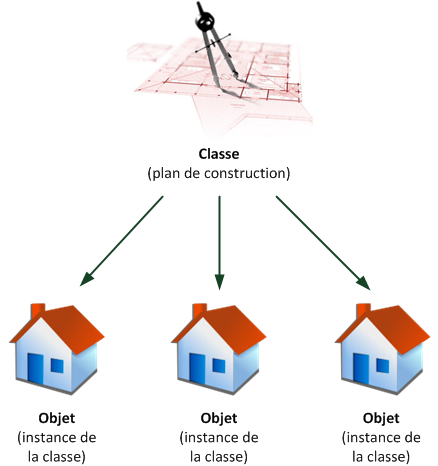
\includegraphics[scale=0.5]{images/objet.png}
\end{center}
\caption{Un plan à partir duquel on crée des objets.}
\end{figure}

Passer de la programmation fonctionnelle\, \footnote{La programmation
fonctionnelle est un paradigme de programmation qui repose sur l'utilisation
majoritaire des fonctions et procédures.} à l'objet fut vraiment difficile. Me
rendant compte que je bloquai énormément, je fis des recherches sur internet
pour trouver un programme équivalent sur lequel je me suis appuyé pour
commencer. M.\bsc{Dubourg} m'a mis sur la voie en me disant d'utiliser des
classes et des méthodes toutes prête de l'entreprise ce qui m'ôtas une grosse
épine du pied, car je n'avais aucune idée de comment je devais faire pour
transcrire une structure de base de données en objet.

Pour utiliser les sources de la société, j'ai dû mettre en place un répertoire
de travail et récupérer les sources via leur ancien gestionnaire de version de
code source. Ceci étant fait il s'agissait maintenant de réussir à faire
fonctionner le site web principal en local sur ma machine. Mon logiciel MAMP\,
\footnote{\emph{Macintosh Apache MySQL PHP} est une combinaison de logiciel.}
m'affichant plein d'erreurs, j'ai décidé d'installer manuellement chacun des
logiciels présents dans celui-ci. Même après cette manipulation le problème
n'avait pas disparu, mon tuteur de stage m'est venu en aide après de longues
heures à chercher en vain. Le problème ce trouvai au niveau de la configuration
de PHP\, \footnote{\emph{Hypertext Preprocessor} est un langage de scripts
libre principalement utilisé pour produire des pages Web dynamiques.} qui
affichait tous les avertissements de manière trop strict, ce qui refusait tout
lancement de la page principale et aussi le fait que je devais vider le cache
de mon navigateur. De nombreuses heures de recherche juste à cause d'un cache
internet pas vidé fut extrêmement frustrant \ldots{}

\section{Comparaison des tables}

%%% arrivé ici %%%

Il a fallu dans un premier temps que je recherche comment extraire le nom d'une
base ainsi que le nom de ses tables. La réponse à cette question est dans la
documentation de MySQL. Une base de données est fournit à l'installation et
elle s'appelle \og information schéma \fg{} . En résumé, c'est une base de
données qui contient les autres bases de données.

Ensuite, j'ai transformé le programme procédural sur plusieurs semaines en
objet, le fait de passer par cette étape intermédiaire m'as permis d'abord de
résoudre le problème algorithmique, puis après me consacrer sur la façon de
l'écrire.

La requête récupérant les données utiles, j'ai dû concevoir un algorithme
capable de comparer les deux tableaux d'objets par rapport à leurs noms :
\begin{itemize}
    \item Si la base de données de référence à une table qui n'est pas dans
    la base de données à mettre à jour, on l'ajoute ;
    \item Si la base de données de mise à jour contient une table qui n'est
    pas dans la base de données de référence, on l'enlève ;
    \item Si les tables comparées sont toutes les deux dans les base de
    données, on compare l'intérieur des tables.
\end{itemize}

J'ai dû revoir mon algorithme plusieurs fois, car la fonction de comparaison
de chaine de caractère \emph{strnatcmp} comparait les mots comme un humain le
ferait, alors que mySQL trie les tables de manière binaire c'est-à-dire les
codes ASCII\, \footnote{\emph{American Standard Code for Information
Interchange.} ou \og Code américain normalisé pour l'échange d'information
\fg{} est la norme de codage de caractères en informatique la plus connue, la
plus ancienne et la plus largement compatible. ASCII contient les caractères
nécessaires pour écrire en anglais.} des caractères ce qui faisait que la
première fonction donner des résultats erronés comme le montre le tableau
ci-dessous.

\begin{center}
\begin{tabular}{|c|c|}
\hline
\textbf{Tri de chaînes standard} & \textbf{Tri de chaînes ordre naturel} \\
\hline
[0] = img1.png & [0] = img1.png \\
\hline
[1] = img10.png & [1] = img2.png \\
\hline
[2] = img12.png & [2] = img10.png \\
\hline
[3] = img2.png & [3] = img12.png \\
\hline
\end{tabular}
\end{center}

\section{Comparaison des champs}

Maintenant que j'étais dans la situation des tables ayant les mêmes noms, il
fallait que je compare le contenu, lui aussi en comparant le nom des champs, il
m'a pas fallut longtemps pour comprendre que l'algorithme était exactement le
même, le plus dur étant de savoir comment j'allais faire pour me répéter le
minimum possible ce qui a bloqué énormément mon avancement pour pas
grand-chose. M.\bsc{Dubourg} constatant que je n'avançais plus m'a conseillé de
faire comme je l'avais appris plutôt que d'essayer de faire de la POO\,
\footnote{\emph{Programmation Orienté Objet.}} tout de suite. Une fois le
script fonctionnel, mais très mal optimisé et peu lisible, mon tuteur m'a guidé
via des annotations et des explications poussées sur la marche à suivre qui
semblai la meilleur. De fil en aiguille le code source est passé d'environ
trois-cent cinquante lignes à cent cinquante.

Ensuite légèrement différent, je devais comparer le contenu des champs des
tables lorsque les champs parcourus avait le même nom, je compare tout
simplement le contenu des champs pour connaitre l'issue finale, à savoir que je
ne pouvais pas décider si les tables était similaire sans avoir balayé tous les
champs et toutes les caractéristiques de ceux-ci.

\section{Affichage du résultat}

Après tout ceci fini est optimisé, j'implémente une nouvelle fonctionnalité qui
permettrait d'afficher un texte lisible qui énonce les différences des deux
bases données. En fonction des résultats obtenus, je génère des balises HTML\,
\footnote{L’ \emph{Hypertext Markup Language} est un langage de balisage conçu
pour représenter les pages web.} et du texte pour que cela soit compréhensible
à l'utilisateur. Ceci étant fait assez rapidement je suis passé à la génération
des requêtes SQL permettant de mettre à jour la base obsolète depuis la base de
référence. C'est à ce stade que j'ai constaté que je ne pourrais pas prendre en
compte les clés étrangères dans mon code à moins de revoir totalement tout le
script. M.\bsc{Dubourg} m'a rassuré sur le fait que l'entreprise n'utilisai pas
le type de base de données myISAM\, \footnote{L'organisation séquentielle
indexée, ou \emph{Indexed Sequential Access Method} en anglais, est un mode
d'organisation des fichiers dans les bases de données.}} et que donc aucune de
leurs tables comportait de clé étrangère, cependant les clés primaires
concaténées restent problématique, car pas imaginer pendant la conception. Nous
avons décidé que la création de ce genre de cas se fera à la main pour pas
repartir de zéro.

Après avoir analysé mes méthodes de génération de phrase lisible et de
requêtes SQL, M.\bsc{Dubourg} m'a présenté un outil nommé \og Smarty \fg{} qui
permet de dissocier la partie traitement de la partie affichage, car il est
vrai que mes méthodes était vraiment très sale. Pour résumer, j'écrivais des
chaînes de caractère dans une seule variable en écrivant les noms des tables ou
des champs, en concaténant le tout avec des balises HTML de saut de ligne un
peu n'importe où. J'ai du parcourir la documentation de Smarty pour comprendre
son fonctionnement, il s'avère que la syntaxe est très particulière mais très
efficace. J'ai terminé par faire de l'agencement sur ma page pour que chaque
ligne lisible par un néophyte soit en face de la ligne en SQL dans un tableau a
deux colonnes tout ceci avec l'aide de Smarty.

\clearpage
